\newpage temp \newpage
\section{Problem Formulation}
Solving the bus charge problem requires knowing when, and on which charger a bus must charge, indicating a solution with two dimensions.  The first dimension represents time continuously from left to right, and the second describes the buses as shown in Fig. \ref{fig:busTime1}.
\begin{figure*}
	\centering
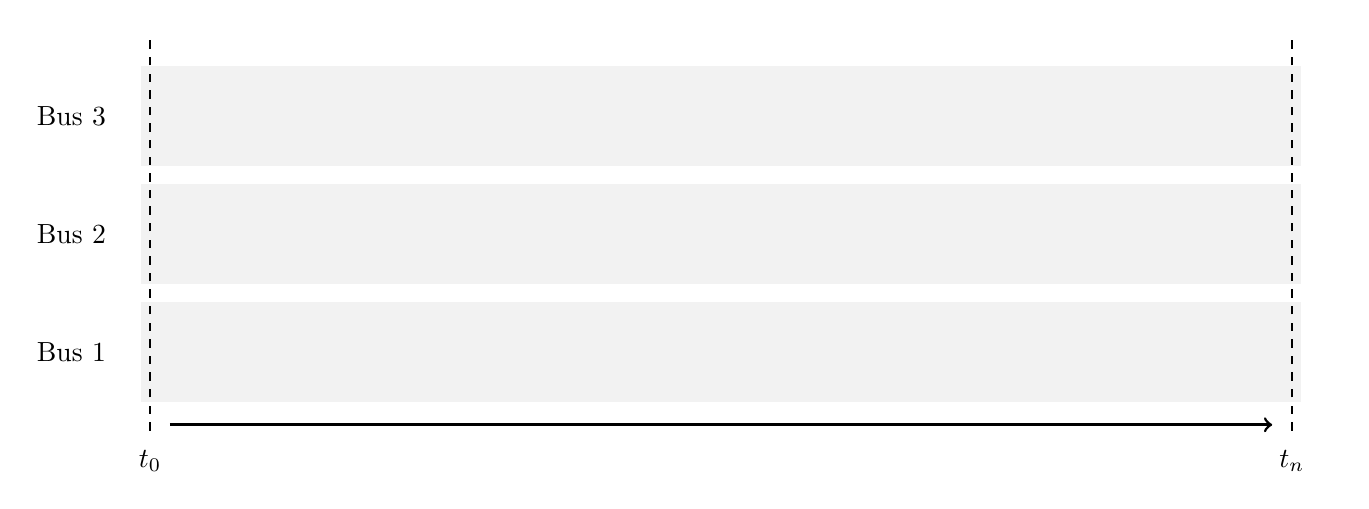
\begin{tikzpicture}
	\node[rectangle, fill=gray!10, minimum width=5.8in, minimum height=0.5in](bus1Box) at (7.75,1){};
	\node(bus1BoxLabel) at (-0.5, 1){Bus 1}; 

	\node[rectangle, fill=gray!10, minimum width=5.8in, minimum height=0.5in](bus2Box) at (7.75,2.5){};
	\node(bus1BoxLabel) at (-0.5, 2.5){Bus 2};

	\node[rectangle, fill=gray!10, minimum width=5.8in, minimum height=0.5in](bus3Box) at (7.75,4){};
	\node(bus1BoxLabel) at (-0.5, 4){Bus 3};

	\node[label=below:$t_0$](origin) at (0.5,0){};
	\node(yAxes) at (15.5,0){};
	\node(xAxes) at (0.5,5){};
	\node[label=below:$t_n$](bottomRight) at (15,0){};
	\node(topRight) at (15,5){};
	\draw[dashed, line width=0.5pt] (origin.center) -- (xAxes.center); 
	\draw[dashed, line width=0.5pt] (bottomRight.center) -- (topRight.center);
	\node(t0) at (0.75,-0.05){};
	\node(tn) at (14.75,-0.05){};
	\draw[->, line width=1pt] (t0.north) -- (tn.north); 
\end{tikzpicture}
	\caption{Description of the bus and time axis}
	\label{fig:busTime1}
\end{figure*}

\par Each bus follows a schedule and is in the station during predefined times. When a bus is in the station, it is available to charge.  Bus availability is described in terms of it's arrival and departure times, where the bus's $n^{\text{th}}$ stop begins at arrival time $n$, or $a_n$ and terminates at the $n^{\text{th}}$ departure time, $d_n$ (see Fig. \ref{fig:busTime2}). 
\begin{figure*}
\centering
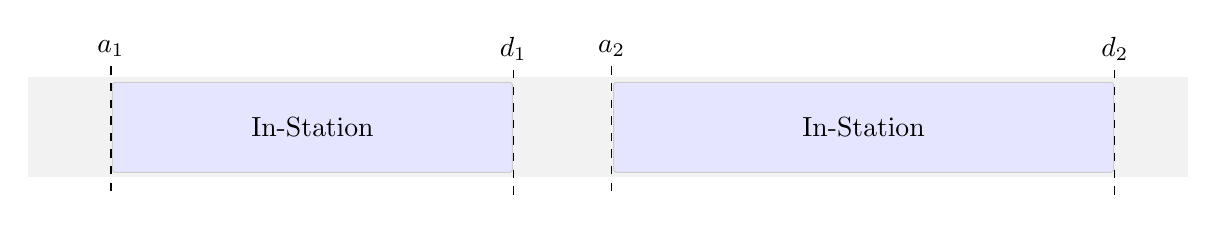
\begin{tikzpicture} 
	\node[rectangle, fill=gray!10, minimum width=5.8in, minimum height=0.5in](busAvail) at (7.75,4){}; 

	\node[rectangle, draw=blue!10!black!20, fill=blue!10, minimum width=2in, minimum height=0.45in, rounded corners=1pt](busAvail1) at (4,4){In-Station};
	\node[rectangle, draw=blue!10!black!20, fill=blue!10, minimum width=2.5in, minimum height=0.45in, rounded corners=1pt](busAvail2) at (11,4){In-Station};

	\node(firstATop) at (1.44,5){$a_1$};
	\node(firstABtm) at (1.44,3.1){};
	\draw[dashed, line width=0.5pt](firstATop) -- (firstABtm.center);
	\node(firstDTop) at (6.55,5){$d_1$};
	\node(firstDBtm) at (6.55,3.1){};
	\draw[dashed, line width=0.5pt](firstDTop) -- (firstDBtm.center);

	\node(secondATop) at (7.8,5){$a_2$};
	\node(secondABtm) at (7.8,3.1){};
	\draw[dashed, line width=0.5pt](secondATop) -- (secondABtm.center);
	\node(secondDTop) at (14.19,5){$d_2$};
	\node(secondDBtm) at (14.19,3.1){};
	\draw[dashed, line width=0.5pt](secondDTop) -- (secondDBtm.center);


\end{tikzpicture}
\caption{Bus availability}
\label{fig:busTime2}
\end{figure*}

\par A bus can be assigned to charge for a time interval where the bus is in the station. The charge start time during the $n^{\text{th}}$ stop is denoted $c_n$ and the stop-charge time is denoted $s_n$ as shown in Fig. \ref{fig:busTime3}. 
\begin{figure*}
\centering
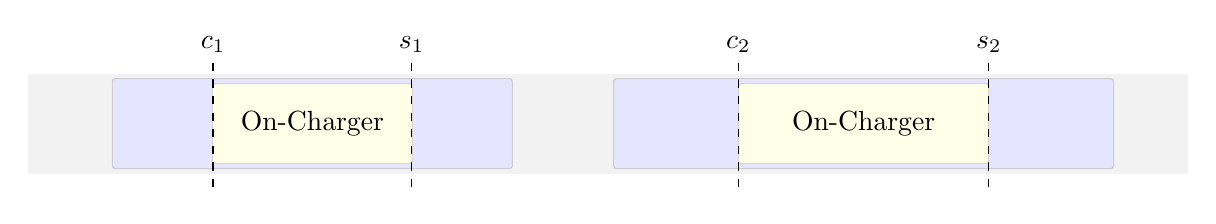
\begin{tikzpicture} 
	\node[rectangle, fill=gray!10, minimum width=5.8in, minimum height=0.5in](busSched) at (7.75,1){}; 

	\node[rectangle, draw=blue!10!black!20, fill=blue!10, minimum width=2in, minimum height=0.45in, rounded corners=1pt](busAvail1) at (4,1){In-Station};
	\node[rectangle, draw=blue!10!black!20, fill=blue!10, minimum width=2.5in, minimum height=0.45in, rounded corners=1pt](busAvail2) at (11,1){In-Station};

	\node[rectangle, draw=yellow!10!black!20, fill=yellow!10, minimum width=1in, minimum height=0.4in, rounded corners=1pt](busAvail1) at (4,1){On-Charger};
	\node[rectangle, draw=yellow!10!black!20, fill=yellow!10, minimum width=1.25in, minimum height=0.4in, rounded corners=1pt](busAvail2) at (11,1){On-Charger};


	\node(firstATop) at (2.74,2){$c_1$};
	\node(firstABtm) at (2.74,0.2){};
	\draw[dashed, line width=0.5pt](firstATop) -- (firstABtm.center);
	\node(firstDTop) at (5.26,2){$s_1$};
	\node(firstDBtm) at (5.26,0.2){};
	\draw[dashed, line width=0.5pt](firstDTop) -- (firstDBtm.center);

	\node(secondATop) at (9.41,2){$c_2$};
	\node(secondABtm) at (9.41,0.2){};
	\draw[dashed, line width=0.5pt](secondATop) -- (secondABtm.center);
	\node(secondDTop) at (12.59,2){$s_2$};
	\node(secondDBtm) at (12.59,0.2){};
	\draw[dashed, line width=0.5pt](secondDTop) -- (secondDBtm.center);


\end{tikzpicture}
\caption{Bus Charging}
\label{fig:busTime3}
\end{figure*}

The relationship between the arrival, departure, and charge intervals for the $i^{\text{th}}$ bus at the $j^{\text{th}}$ stop can be expressed as a set of inequality constraints such that
\begin{align}
	a_{ij} &< c_{ij} \\
	c_{ij} &< s_{ij} \\
	s_{ij} &< d_{ij}
\end{align}
Which can be expressed in standard form as
\begin{align}
	-c_{ij} &< -a_{ij}\\
	c_{ij} - s_{ij} &< 0\\
	s_{ij} &< d_{ij}
\end{align}
and finally, 
\begin{align}\label{eqn:timeConstraint}
	\begin{bmatrix} -1 & 0 \\
	                 1 & -1 \\
		0 & 1\end{bmatrix} \begin{bmatrix} c_{ij} \\ s_{ij}\end{bmatrix} \le \begin{bmatrix}-a_{ij} \\ 0 \\ d_{ij} \end{bmatrix}.
\end{align}

\par A charge plan can be formulated by reserving time slots at chargers when buses need to charge (see Fig. \ref{fig:busTime4}).
\begin{figure*}
	\centering
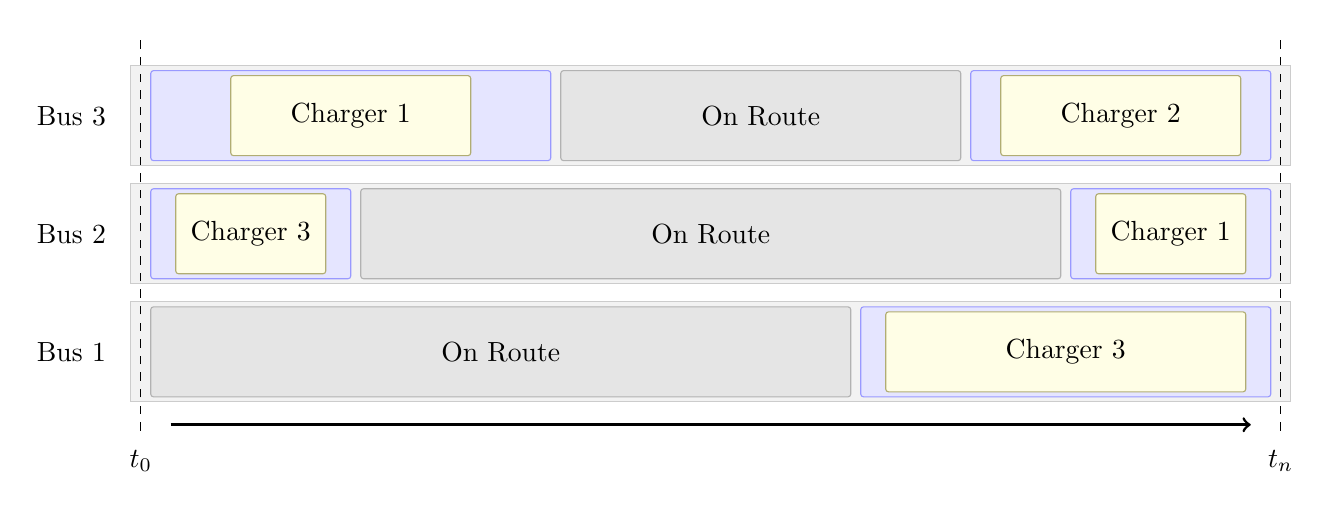
\begin{tikzpicture}
	\node[rectangle, draw=gray!40, fill=gray!10, minimum width=5.8in, minimum height=0.5in](charger1Box) at (3in,1){};
	\node(bus1BoxLabel) at (-0.5, 1){Bus 1}; 

	\node[rectangle, draw=gray!40, fill=gray!10, minimum width=5.8in, minimum height=0.5in](charger2Box) at (3in,2.5){};
	\node(bus1BoxLabel) at (-0.5, 2.5){Bus 2};

	\node[rectangle, draw=gray!40, fill=gray!10, minimum width=5.8in, minimum height=0.5in](charger3Box) at (3in,4){};
	\node(bus1BoxLabel) at (-0.5, 4){Bus 3};

	\node[label=below:$t_0$](origin) at (0.15in,0){};
	\node(xAxes) at (0.15in,5){};
	\node[label=below:$t_n$](bottomRight) at (5.85in,0){};
	\node(topRight) at (5.85in,5){};
	\draw[dashed, line width=0.5pt] (origin.center) -- (xAxes.center); 
	\draw[dashed, line width=0.5pt] (bottomRight.center) -- (topRight.center);
	\node(t0) at (0.3in,-0.05){};
	\node(tn) at (5.7in,-0.05){};
	\draw[->, line width=1pt] (t0.north) -- (tn.north); 

	% draw bus 3 boxes
	\node[rectangle, draw=blue!40, fill=blue!10, minimum width=2in, minimum height=0.45in, rounded corners=1pt](bus1Avail1) at (1.2in,4){};
	\node[rectangle, draw=yellow!50!black!70, fill=yellow!10, minimum width=1.2in, minimum height=0.4in, rounded corners=1pt](bus1Time1) at (1.2in,4){Charger 1};

	\node[rectangle, draw=black!30, fill=black!10, minimum width=2in, minimum height=0.45in, rounded corners=1pt](bus2Time1) at (3.25in,4){On Route};

	\node[rectangle, draw=blue!40, fill=blue!10, minimum width=1.5in, minimum height=0.45in, rounded corners=1pt](bus1Avail1) at (5.05in,4){};
	\node[rectangle, draw=yellow!50!black!70, fill=yellow!10, minimum width=1.2in, minimum height=0.40in, rounded corners=1pt](bus3Time1) at (5.05in,4){Charger 2};

	% draw bus 2 boxes
	\node[rectangle, draw=blue!40, fill=blue!10, minimum width=1in, minimum height=0.45in, rounded corners=1pt](bus1Avail1) at (0.7in,2.5){};
	\node[rectangle, draw=yellow!50!black!70, fill=yellow!10, minimum width=0.75in, minimum height=0.4in, rounded corners=1pt](free1) at (0.7in,2.5){Charger 3};

	\node[rectangle, draw=black!30, fill=black!10, minimum width=3.5in, minimum height=0.45in, rounded corners=1pt](bus3Time2) at (3.0in,2.5){On Route};

	\node[rectangle, draw=blue!40, fill=blue!10, minimum width=1.0in, minimum height=0.45in, rounded corners=1pt](bus1Avail1) at (5.3in,2.5){};
	\node[rectangle, draw=yellow!50!black!70, fill=yellow!10, minimum width=0.75in, minimum height=0.4in, rounded corners=1pt](free2) at (5.3in,2.5){Charger 1};

	% draw bus 1 boxes 
	\node[rectangle, draw=black!30!, fill=black!10, minimum width=3.5in, minimum height=0.45in, rounded corners=1pt](bus3Time2) at (1.95in,1){On Route}; 

	\node[rectangle, draw=blue!40, fill=blue!10, minimum width=2.05in, minimum height=0.45in, rounded corners=1pt](bus1Avail1) at (4.775in,1){};
	\node[rectangle, draw=yellow!50!black!70, fill=yellow!10, minimum width=1.8in, minimum height=0.4in, rounded corners=1pt](bus1Time2) at (4.775in,1){Charger 3};
\end{tikzpicture}
	\caption{Reserving time slots on chargers}
	\label{fig:busTime4}
\end{figure*}

	Note how there are several decisions that go into the charge schedule, which is made up to which bus charges at which charger at which time. 
	\par The variables for time have already been discussed in equation \ref{eqn:timeConstraint}, but variables for which charger have not been given.  Let $\sigma_{ijk}$ be a binary variable that is $1$ when bus $i$ charges during the $j^{\text{th}}$ stop at charger $k$. Because a bus can only charge at one charger at a time, we also constraint $\sigma$ such that
	\begin{equation}
		\begin{aligned}
			\sum_k \sigma_{ijk} \le 1 \ \forall i,j
		\end{aligned}
	\end{equation}
	$\sigma_{ijk}$ is necessary to eliminate situations where more then one bus is assigned to a charger at the same time. Note that this can only happen when $a_{ij}$ for bus $j$ is less than $d_{i^{'}j^{'}}$ for bus $j^{'}$ as shown in Fig. \ref{fig:potentialOverlap}. Charging overlap can be avoided by constraining
	\begin{figure}
	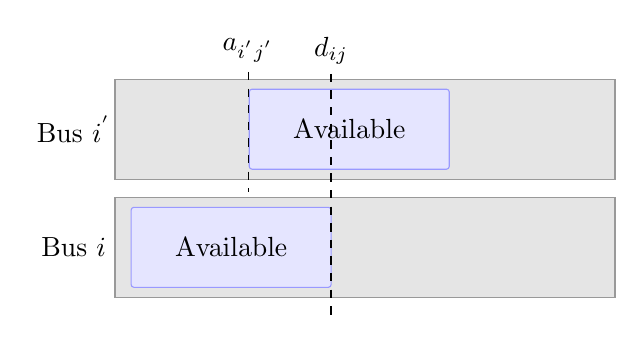
\begin{tikzpicture} 
		\node[rectangle, draw=black!40, fill=black!10, minimum width=2.5in, minimum height=0.5in](charger1Box) at (3.2,1){};
		\node(bus1BoxLabel) at (-0.5, 1){Bus $i$}; 
		\node[rectangle, draw=black!40, fill=black!10, minimum width=2.5in, minimum height=0.5in](charger2Box) at (3.2,2.5){};
		\node(bus1BoxLabel) at (-0.5, 2.5){Bus $i^{'}$};
		\node[rectangle, draw=blue!40, fill=blue!10, minimum width=1in, minimum height=0.4in, rounded corners=1pt] at (1.5,1){Available};
		\node[rectangle, draw=blue!40, fill=blue!10, minimum width=1in, minimum height=0.4in, rounded corners=1pt] at (3,2.5){Available};
		\node(aJPrimeHigh) at (1.72,3.5){$a_{i^{'}j^{'}}$};
		\node(aJPrimeLow) at (1.72,1.7){};
		\node(dJHigh) at (2.77,3.5){$d_{ij}$};
		\node(dJLow) at (2.77,0.0){};
		\draw[dashed, line width=0.5pt] (aJPrimeHigh) -- (aJPrimeLow.center);
		\draw[dashed, line width=0.5pt] (dJHigh) -- (dJLow);
	\end{tikzpicture}
	\caption{Potential Overlap}
	\label{fig:potentialOverlap}
\end{figure}


	
	\begin{align}\label{eqn:overlapConstraints1}
	c_{i^{'}j^{'}} > s_{ij}.
\end{align}
However, this constraint is only necessary when both bus stops are designated for charging. This can be remedied as
	\begin{align}\label{eqn:overlapConstraints2}
		c_{i^{'}j^{'}} - s_{ij} > M\left[(\sigma_{i^{'}j^{'}k^{'}} + \sigma_{ijk}) - 2\right]
	\end{align}
	Where $M = 2\cdot\text{nTime}$. When $(\sigma_{i^{'}j^{'}k^{'}} + \sigma_{ijk}) < 2$, then equation \ref{eqn:overlapConstraints2} is trivially satisfied for all values of $c_{i^{'}j^{'}}$ and $s_{ij}$ and when $\sigma_{i^{'}j^{'}k^{'}} = \sigma_{ijk} = 1$, equation \ref{eqn:overlapConstraints2} simplifies to equation \ref{eqn:overlapConstraints1}. Equation \ref{eqn:overlapConstraints1} can be expressed in standard form as 
	\begin{align}\label{eqn:overlapConstraints3}
		c_{i^{'}j^{'}} - s_{ij} - M\sigma_{i^{'}j^{'}k^{'}} - M\sigma_{ijk} &\ge -2M \\
		-c_{i^{'}j^{'}} + s_{ij} + M\sigma_{i^{'}j^{'}k^{'}} + M\sigma_{ijk} &\le 2M \\
		\begin{bmatrix} -1 & 1 & M & M\end{bmatrix} \begin{bmatrix}c_{i^{'}j^{'}}\\ s_{ij} \\ \sigma_{i^{'}j^{'}k^{'}}\\ \sigma{ijk} \end{bmatrix} &\le 2M
	\end{align}
	The constraints in equation \ref{eqn:overlapConstraints3} can be repeated for all instances where overlap is possible and concatenated into a single matrix such that
	\begin{equation}
		A\mathbf{y} \le \mathbf{1}\cdot 2M
	\end{equation}



